\documentclass[10pt]{article}
\usepackage{fullpage,enumitem,amsmath,amssymb,graphicx,listings,tikz,bbm,xcolor}
\setlength{\parindent}{0pt}

\begin{document}

\begin{center}
{\Large \textbf{Homework 6: Scheduling}}

\begin{tabular}{rl}
\\
Course: & CS 221 Spring 2019 \\
Name: & Bryan Yaggi
\end{tabular}
\end{center}

What courses should you take in a given quarter? Answering this question requires balancing your interests, satisfying prerequisite chains, graduation requirements, availability of courses; this can be a complex tedious process. In this assignment, you will write a program that does automatic course scheduling for you based on your preferences and constraints. The program will cast the course scheduling problem (CSP) as a constraint satisfaction problem (CSP) and then use backtracking search to solve that CSP to give you your optimal course schedule.
\smallskip

You will first get yourself familiar with the basics of CSPs in Problem 0. In Problem 1, you will implement two of the three heuristics you learned from the lectures that will make CSP solving much faster. In Problem 2, you will add a helper function to reduce n-ary factors to unary and binary factors. Lastly, in Problem 3, you will create the course scheduling CSP and solve it using the code from previous parts. 

\section*{\normalsize Problem 0: CSP Basics}

\begin{enumerate}[label=(\alph*)]

  \item Let's create a CSP. Suppose you have $n$ light bulbs, where each light bulb $i = 1, \dots, n$ is initially off. You also have $m$ buttons which control the lights. For each button $j = 1, \dots, m$, we know the subset $T_j \subseteq \{1, \dots, n\}$ of light bulbs that it controls. When button $j$ is pressed, it toggles the state of each light bulb in $T_j$ (For example, if $3 \in T_j$ and light bulb 3 is off, then after the button is pressed, light bulb 3 will be on, and vice versa).
  
  Your goal is to turn on all the light bulbs by pressing a subset of the buttons. Construct a CSP to solve this problem. Your CSP should have $m$ variables and $n$ constraints. For this problem only, you can use n-ary constraints. Describe your CSP precisely and concisely. You need to specify the variables with their domain, and the constraints with their scope and expression. Make sure to include $T_j$ in your answer.
  
  There are $m$ variables, one for each button. The domain consists of 1 or 0, indicating whether the button is pressed or not.
  $$X = (X_1, \dots, X_m), where \ X_j \in \{0, 1\}$$
  
  There are $n$ factors, one for each light. The factor will be 1 if the number of pressed buttons controlling the light is odd.
  $$f_i = \mathbbm{1}\left[\left(\sum_{j : i \in T_j}^{m} X_j \right) \mod 2\right]$$
  
  \item Let's consider a simple CSP with 3 variables and 2 binary factors:
  
  \begin{center}
	  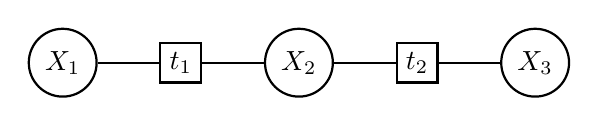
\begin{tikzpicture}
			\begin{scope}[every node/.style={circle,thick,draw}]
	    		\node (X1) at (3,0) {$X_1$};
	    		\node (X2) at (6,0) {$X_2$};
	    		\node (X3) at (9,0) {$X_3$};
			\end{scope}
			\begin{scope}[every node/.style={rectangle,thick,draw}]
	    		\node (t1) at (4.5,0) {$t_1$};
	    		\node (t2) at (7.5,0) {$t_2$};
			\end{scope}
	
			\begin{scope}[every edge/.style={draw=black,thick}]
				\path [-] (X1) edge node {} (t1);	    		
	    		\path [-] (t1) edge node {} (X2);
	    		\path [-] (X2) edge node {} (t2);
	    		\path [-] (t2) edge node {} (X3);
			\end{scope}
		\end{tikzpicture}
	\end{center}
	
	where $X_1, X_2, X_3 \in \{ 0, 1 \}$ and $t_1, t_2$ are XOR functions (that is $t_1(X) = X_1 \oplus X_2$ and $t_2(X) = X_2 \oplus X_3$).
	
	\begin{enumerate}[label=\roman*.]
		\item How many consistent assignments are there for this CSP?
		
		\begin{tabular}{c c c c c c}
		$X_1$ & $X_2$ & $X_3$ & $t_1$ & $t_2$ & $weight$\\
		\hline
  		$0$ & $0$ & $0$ & $0$ & $0$ & $0$\\
  		$1$ & $0$ & $0$ & $1$ & $0$ & $0$\\
  		$0$ & $1$ & $0$ & $1$ & $1$ & $1$\\
  		$1$ & $1$ & $0$ & $0$ & $1$ & $0$\\
  		$0$ & $0$ & $1$ & $0$ & $1$ & $0$\\
  		$1$ & $0$ & $1$ & $1$ & $1$ & $1$\\
  		$0$ & $1$ & $1$ & $1$ & $0$ & $0$\\
  		$1$ & $1$ & $1$ & $0$ & $0$ & $0$\\
  		\end{tabular}
  		
  		There are 2 consistent assignments: $x = \{ X_1 = 0, X_2 = 1, X_3 = 0 \}$ and $x = \{ X_1 = 1, X_2 = 0, X_3 = 1 \}$.
		
		\item To see why variable ordering is important, let's use backtracking search to solve the CSP without using any heuristics (MCV, LCV, AC-3) or lookahead. How many times will \texttt{backtrack()} be called to get all consistent assignments if we use the fixed ordering $X_1, X_3, X_2$? Draw the call stack for \texttt{backtrack()}. (You should use the Backtrack algorithm from the slides. The initial arguments are $x = \emptyset, w = 1$, and the original Domain.)
		
		In the code, this number will be stored in \texttt{BacktrackingSearch.numOperations}.
		
		Use domain ordering $Domain = \{ 0, 1 \}$. The top of the stack is on the bottom.
		
		\begin{tabular}{l}
		\textcolor{black}{\texttt{backtrack($x = \emptyset$, $w = 1$)}}\\
		\textcolor{black}{\texttt{backtrack($x = \{ X_1 = 0 \}$, $w = 1$)}}\\
		\textcolor{black}{\texttt{backtrack($x = \{ X_1 = 0, X_3 = 0 \}$, $w = 1$)}}\\
		\textcolor{black}{\texttt{backtrack($x = \{ X_1 = 0, X_3 = 0, X_2 = 1 \}$, $w = 1$)}} \textit{consistent assignment found}\\
		\hline
		\textcolor{gray}{\texttt{backtrack($x = \emptyset$, $w = 1$)}}\\
		\textcolor{gray}{\texttt{backtrack($x = \{ X_1 = 0 \}$, $w = 1$)}}\\
		\texttt{backtrack($x = \{ X_1 = 0, X_3 = 1 \}$, $w = 1$)}\\
		\hline
		\textcolor{gray}{\texttt{backtrack($x = \emptyset$, $w = 1$)}}\\
		\texttt{backtrack($x = \{ X_1 = 1 \}$, $w = 1$)}\\
		\texttt{backtrack($x = \{ X_1 = 1, X_3 = 0 \}$, $w = 1$)}\\
		\hline
		\textcolor{gray}{\texttt{backtrack($x = \emptyset$, $w = 1$)}}\\
		\textcolor{gray}{\texttt{backtrack($x = \{ X_1 = 1 \}$, $w = 1$)}}\\
		\texttt{backtrack($x = \{ X_1 = 1, X_3 = 1 \}$, $w = 1$)}\\
		\texttt{backtrack($x = \{ X_1 = 1, X_3 = 1, X_2 = 0 \}$, $w = 1$)} \textit{consistent assignment found}\\
  		\end{tabular}
  		
  		\texttt{backtrack()} is called 9 times.
		
		\item To see why lookahead can be useful, let's do it again with the ordering $X_1, X_3, X_2$ and AC-3. How many times will Backtrack be called to get all consistent assignments? Draw the call stack for \texttt{backtrack()}.
		
		\begin{tabular}{l}
		\textcolor{black}{\texttt{backtrack($x = \emptyset$, $w = 1$)}}\\
		\textcolor{black}{\texttt{backtrack($x = \{ X_1 = 0 \}$, $w = 1$)}} $Domain_3 = \{ 0 \}$ $Domain_2 = \{ 1 \}$ \\
		\textcolor{black}{\texttt{backtrack($x = \{ X_1 = 0, X_3 = 0 \}$, $w = 1$)}} $Domain_2 = \{ 1 \}$\\
		\textcolor{black}{\texttt{backtrack($x = \{ X_1 = 0, X_3 = 0, X_2 = 1 \}$, $w = 1$)}} \textit{consistent assignment found}\\
		\hline
		\textcolor{gray}{\texttt{backtrack($x = \emptyset$, $w = 1$)}}\\
		\texttt{backtrack($x = \{ X_1 = 1 \}$, $w = 1$)} $Domain_3 = \{ 1 \}$ $Domain_2 = \{ 0 \}$\\
		\texttt{backtrack($x = \{ X_1 = 1, X_3 = 1 \}$, $w = 1$)} $Domain_2 = \{ 0 \}$\\
		\texttt{backtrack($x = \{ X_1 = 1, X_3 = 1, X_2 = 0 \}$, $w = 1$)} \textit{consistent assignment found}\\
  		\end{tabular}
  		
  		\texttt{backtrack()} is called 7 times.
	\end{enumerate}
	
	\item coding

\end{enumerate}

\section*{\normalsize Problem 1: CSP Solving}

\begin{enumerate}[label=(\alph*)]

  \item coding
  
  \item coding
  
  \item coding

\end{enumerate}

\section*{\normalsize Problem 2: Handling N-ary Factors}

So far, our CSP solver only handles unary and binary factors, but for course scheduling (and really any non-trivial application), we would like to define factors that involve more than two variables. It would be nice if we could have a general way of reducing n-ary constraint to unary and binary constraints. In this problem, we will do exactly that for two types of n-ary constraints.
\smallskip

Suppose we have boolean variables $X_1, X_2, X_3$, where $X_i$ represents whether the $i$-th course is taken. Suppose we want to enforce the constraint that $Y = X_1 \vee X_2 \vee X_3$, that is, $Y$ is a boolean representing whether at least one course has been taken. For reference, in \texttt{util.py}, the function \texttt{get\_or\_variable()} does such a reduction. It takes in a list of variables and a target value, and returns a boolean variable with domain $[True, False]$ whose value is constrained to the condition of having at least one of the variables assigned to the target value. For example, we would call \texttt{get\_or\_variable()} with arguments $(X_1, X_2, X_3, True)$, which would return a new (auxiliary) variable $X_4$, and then add another constraint $[X_4 = True]$.
\smallskip

The second type of n-ary factors are constraints on the sum over $n$ variables. You are going to implement reduction of this type but let's first look at a simpler problem to get started:

\begin{enumerate}[label=(\alph*)]

  \item Suppose we have a CSP with three variables $X_1, X_2, X_3$ with the same domain $\{ 0, 1, 2 \}$ and a ternary constraint $[X_1 + X_2 + X_3 \leq K]$. How can we reduce this CSP to one with only unary and/or binary constraints? Explain what auxiliary variables we need to introduce, what their domains are, what unary/binary factors you'll add, and why your scheme works. Add a graph if you think that'll better explain your scheme.
  
  Define a new variables $A_i, B_i$.
	\begin{align*}
		A_i &= A_{i-1} + X_i, A_0 = 0\\
		B_i &= (A_{i-1}, A_i)\\
  		Domain(B_i) &= \{ (x,y) : 0 \leq x \leq 6, 0 \leq y \leq 6, x \in \mathbb{Z}, y \in \mathbb{Z} \}
	\end{align*}	  
  
  
  Factors:
  \begin{itemize}
  		\item $\mathbbm{1}[B_1[0] = 0]$
  		\item $\mathbbm{1}[B_3[1] \leq K]$
  		\item $\mathbbm{1}[B_i[0] = B_{i-1}[1]]$
  		\item $\mathbbm{1}[B_i[1] = B_{i-1} + X_i]$
  \end{itemize}
  
  \begin{center}
	  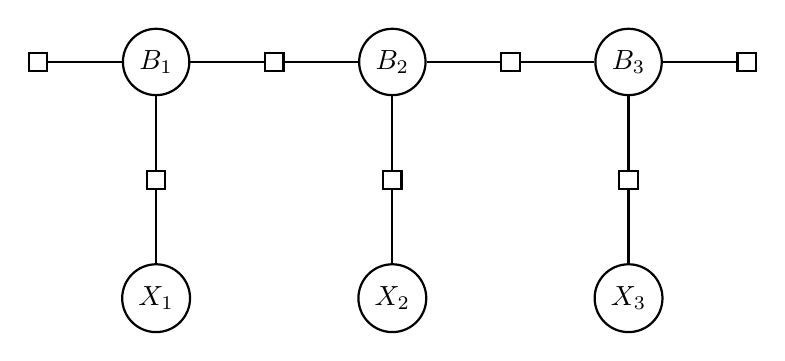
\begin{tikzpicture}
			\begin{scope}[every node/.style={circle,thick,draw}]
	    		\node (B1) at (3,0) {$B_1$};
	    		\node (B2) at (6,0) {$B_2$};
	    		\node (B3) at (9,0) {$B_3$};
	    		\node (X1) at (3,-3) {$X_1$};
	    		\node (X2) at (6,-3) {$X_2$};
	    		\node (X3) at (9,-3) {$X_3$};
			\end{scope}
			\begin{scope}[every node/.style={rectangle,thick,draw}]
				\node (t0) at (1.5,0)	 {};  		
	    		\node (t1) at (4.5,0) {};
	    		\node (t2) at (7.5,0) {};
	    		\node (t3) at (10.5,0) {};
	    		\node (t4) at (3,-1.5) {};
	    		\node (t5) at (6,-1.5) {};
	    		\node (t6) at (9,-1.5) {};
			\end{scope}
	
			\begin{scope}[every edge/.style={draw=black,thick}]
				\path [-] (t0) edge node {} (B1);	    		
	    		\path [-] (B1) edge node {} (t1);
	    		\path [-] (t1) edge node {} (B2);
	    		\path [-] (B2) edge node {} (t2);
	    		\path [-] (t2) edge node {} (B3);
	    		\path [-] (B3) edge node {} (t3);
	    		\path [-] (B1) edge node {} (t4);	    		
	    		\path [-] (t4) edge node {} (X1);
	    		\path [-] (B2) edge node {} (t5);
	    		\path [-] (t5) edge node {} (X2);
	    		\path [-] (B3) edge node {} (t6);
	    		\path [-] (t6) edge node {} (X3);
			\end{scope}
		\end{tikzpicture}
	\end{center}
  
  \item coding

\end{enumerate}

\section*{\normalsize Problem 3: Course Scheduling}

In this problem, we will apply your weighted CSP solver to the problem of course scheduling. We have scraped a subset of courses that are offered from Stanford's Bulletin. For each course in this dataset, we have information on which quarters it is offered, the prerequisites (which may not be fully accurate due to ambiguity in the listing), and the range of units allowed. You can take a look at all the courses in \texttt{courses.json}. Please refer to \texttt{util.Course} and \texttt{util.CourseBulletin} for more information. 

\begin{enumerate}[label=(\alph*)]

  \item coding
  
  \item coding
  
  \item Now try to use the course scheduler for the winter and spring (and next year if applicable). Create your own \texttt{profile.txt} and then run the course scheduler:

	\texttt{python run\_p3.py profile.txt}

	You might want to turn on the appropriate heuristic flags to speed up the computation. Does it produce a reasonable course schedule? Please include your \texttt{profile.txt} and the best schedule in your writeup; we're curious how it worked out for you!

	\texttt{profile.txt}\\
	\texttt{-----------}\\
	\texttt{minUnits 3}\\
	\texttt{maxUnits 5}\\
	\texttt{taken STATS116}\\
	\texttt{taken CS106A}\\
	\texttt{taken CS106B}\\
	\texttt{taken CS103}\\
	\texttt{taken CS107}\\
	\texttt{taken CS109}\\
	\texttt{taken CS110}\\
	\texttt{taken CS221}\\
	\texttt{request CS161 weight 2}\\
	\texttt{request CS231N weight 2}\\
	\texttt{request CS229}\\
	\texttt{request CS230}\\
	\texttt{request CS234}\\
	\texttt{-----------}

	Resulting best schedule:\\
		\begin{tabular}{l l l}
			Quarter & Units & Course\\
			\hline
	  		Sum2019 & 5 & CS161\\
	  		Aut2019 & 4 & CS229\\
	  		Win2020 & 3 & CS234\\
	  		Spr2020 & 4 & CS231N\\
	  	\end{tabular}
	  	
	  	Note: I added CS230, CS231N, and CS234 to \texttt{courses.json}.

\end{enumerate}
\iffalse
\section*{\normalsize Problem 4: Evaluation Function (Extra Credit)}

So far, we've seen how MDP algorithms can take an MDP which describes the full dynamics of the game and return an optimal policy. But suppose you go into a casino, and no one tells you the rewards nor the transitions. We will see how reinforcement learning can allow you to play the game and learn its rules and strategy at the same time!

\begin{enumerate}[label=(\alph*)]

  \item coding
  
  \item Clearly describe your evaluation function. What is the high-level motivation? Also talk about what else you tried, what worked and what didn't. Please write your thoughts in \texttt{pacman.pdf} (not in code comments).
  
  The overall strategy is as follows. If there are scared ghosts, chase the nearest scared ghost. If there are no scared ghosts but there are remaining capsules, chase the nearest capsule. If there are no scared ghosts and all capsules are gone, chase the nearest food. Features included the score and reciprocal of the distance to nearest objective. Distance is calculated using the \texttt{manhattanDistance} function in \texttt{util.py}. A penalty is added if a capsule is collected while a scared ghost is present.
		
\end{enumerate}
\fi
\end{document}
